\documentclass[hyperref={pdfpagelabels=true}]{beamer}
\usepackage{lmodern}
\usepackage{textpos}
\usepackage{amsmath}
\usepackage{tcolorbox}
\usepackage{graphicx,xcolor}
\usepackage{listings}
\usepackage{pifont}
\usepackage{booktabs}% http://ctan.org/pkg/booktabs
\usepackage[final]{pdfpages}
\usepackage{multimedia}
\usepackage{attachfile}
\usepackage{media9}
\usepackage{wrapfig}


%\attachfile{\jobname.tex}
%%----------------attach using embedfile-----------------------------------
\usepackage{embedfile}
%\immediate\write18{zip -j -e -P mypassword -r \jobname.tex.zeep \jobname.tex}
%\embedfile{\jobname.tex}
%%----------------attach using navigator-----------------------------------
\usepackage{navigator}
\usepackage{color} %red, mygreen, blue, yellow, cyan, magenta, black, white
\definecolor{mygreen}{RGB}{28,172,0} % color values Red, mygreen, Blue
\definecolor{mygree}{RGB}{95,135,185} % color values Red, mygreen, Blue
\definecolor{mylilas}{RGB}{170,55,241}
\usepackage[utf8]{inputenc} % UFT8 - danske bogstaver
\usepackage[T1]{fontenc}
\usepackage[version=3]{mhchem}
\usepackage{tikz}
%\usepackage{xcolor}
\usepackage{xparse}
\usepackage{xmpmulti}
\usetikzlibrary{shapes.geometric, arrows}
\usetikzlibrary{shapes,snakes}
\usetikzlibrary{chains,fit,shapes}
\usepackage{amssymb}
\usepackage{ifthen}
\usepackage{animate}
\usetikzlibrary{shapes,arrows}
\usepackage{amsmath,bm,times}
\usetikzlibrary[topaths]
\usetikzlibrary{decorations.pathmorphing} % noisy shapes
\usetikzlibrary{fit}					% fitting shapes to coordinates
\usetikzlibrary{backgrounds}	% drawing the background after the foreground
\usepackage{lipsum}   % To generate test text
\usepackage{framed}
\usepackage{ifthen}
\usepackage{geometry}% for screen preview
\sloppy
\definecolor{lightgray}{gray}{0.5}
\setlength{\parindent}{0pt}
\usepackage{amsthm}
\usepackage{amsfonts}
\usetikzlibrary{decorations.pathmorphing,calc,shadows.blur,shadings}
\newcounter{mathseed}
\setcounter{mathseed}{3}
\pgfmathsetseed{\arabic{mathseed}} % To have predictable results
% Define a background layer, in which the parchment shape is drawn
\pgfdeclarelayer{background}
\pgfsetlayers{background,main}
\usetikzlibrary{matrix,shapes,arrows,positioning,chains}

% This is the base for the fractal decoration. It takes a random point between the start and end, and
% raises it a random amount, thus transforming a segment into two, connected at that raised point
% This decoration can be applied again to each one of the resulting segments and so on, in a similar
% way of a Koch snowflake.
\pgfdeclaredecoration{irregular fractal line}{init}
{
  \state{init}[width=\pgfdecoratedinputsegmentremainingdistance]
  {
    \pgfpathlineto{\pgfpoint{random*\pgfdecoratedinputsegmentremainingdistance}{(random*\pgfdecorationsegmentamplitude-0.02)*\pgfdecoratedinputsegmentremainingdistance}}
    \pgfpathlineto{\pgfpoint{\pgfdecoratedinputsegmentremainingdistance}{0pt}}
  }
}


% define some styles
\tikzset{
   paper/.style={draw=black!10, blur shadow, every shadow/.style={opacity=1, black}, shade=bilinear interpolation,
                 lower left=black!10, upper left=black!5, upper right=white, lower right=black!5, fill=none},
   irregular cloudy border/.style={decoration={irregular fractal line, amplitude=0.2},
           decorate,
     },
   irregular spiky border/.style={decoration={irregular fractal line, amplitude=-0.2},
           decorate,
     },
   ragged border/.style={ decoration={random steps, segment length=7mm, amplitude=2mm},
           decorate,
   }
}

\def\tornpaper#1{%
\ifthenelse{\isodd{\value{mathseed}}}{%
\tikz{
  \node[inner sep=1em] (A) {#1};  % Draw the text of the node
  \begin{pgfonlayer}{background}  % Draw the shape behind
  \fill[paper] % recursively decorate the bottom border
     \pgfextra{\pgfmathsetseed{\arabic{mathseed}}\addtocounter{mathseed}{1}}%
      {decorate[irregular cloudy border]{decorate{decorate{decorate{decorate[ragged border]{
        (A.north west) -- (A.north east)
      }}}}}}
      -- (A.south east)
     \pgfextra{\pgfmathsetseed{\arabic{mathseed}}}%
      {decorate[irregular spiky border]{decorate{decorate{decorate{decorate[ragged border]{
      -- (A.south west)
      }}}}}}
      -- (A.north west);
  \end{pgfonlayer}}
}{%
\tikz{
  \node[inner sep=1em] (A) {#1};  % Draw the text of the node
  \begin{pgfonlayer}{background}  % Draw the shape behind
  \fill[paper] % recursively decorate the bottom border
     \pgfextra{\pgfmathsetseed{\arabic{mathseed}}\addtocounter{mathseed}{1}}%
      {decorate[irregular spiky border]{decorate{decorate{decorate{decorate[ragged border]{
        (A.north east) -- (A.north west)
      }}}}}}
      -- (A.south west)
     \pgfextra{\pgfmathsetseed{\arabic{mathseed}}}%
      {decorate[irregular cloudy border]{decorate{decorate{decorate{decorate[ragged border]{
      -- (A.south east)
      }}}}}}
      -- (A.north east);
  \end{pgfonlayer}}
}}
% A counter, since TikZ is not clever enough (yet) to handle
% arbitrary angle systems.
\newcount\mycount
%\usepackage{asymptote}
\newcommand{\mx}[1]{\mathbf{\bm{#1}}} % Matrix command
\newcommand{\vc}[1]{\mathbf{\bm{#1}}} % Vector command
\newcounter{angle}
\setcounter{angle}{0}

\usetheme[hideothersubsections,hideothersubsubsections]{Hannover}
\usecolortheme{sidebartab,wolverine,spruce,seagull}
%\usecolortheme{sidebartab,seagull,fly,solarized}%,sidebartab,wolverine,spruce,seagul}
\definecolor{UniBlue}{RGB}{83,121,170}
\setbeamercolor{title}{fg=UniBlue}
\setbeamercolor{frametitle}{fg=UniBlue}
\setbeamercolor{structure}{fg=UniBlue}
%\useoutertheme{infolines}

\definecolor{mygray}{gray}{0.6}

\tikzstyle{mybox1} = [draw=red, fill=blue!20, very thick,
    rectangle, rounded corners, inner sep=10pt, inner ysep=10pt]
\tikzstyle{fancytitle1} =[fill=red, text=white]


\tikzstyle{mybox2} = [draw=mygreen, fill=gray!20, very thick,
    rectangle, rounded corners, inner sep=10pt, inner ysep=10pt]
\tikzstyle{fancytitle2} =[fill=mygreen, text=white]

\tikzstyle{mybox} = [draw=blue, fill=green!20, very thick,
    rectangle, rounded corners, inner sep=10pt, inner ysep=20pt]
\tikzstyle{fancytitle} =[fill=blue, text=white, ellipse]

\tikzstyle{startstop} = [rectangle, rounded corners, minimum width=3cm, minimum height=1cm,text centered, draw=black, fill=red!30]
\tikzstyle{io} = [trapezium, trapezium left angle=70, trapezium right angle=110, minimum width=3cm, minimum height=1cm, text centered, draw=black, fill=blue!30]
\tikzstyle{process} = [rectangle, minimum width=3cm, minimum height=1cm, text centered, draw=black, fill=orange!30]
\tikzstyle{decision} = [diamond, minimum width=3cm, minimum height=1cm, text centered, draw=black, fill=green!30]
\tikzstyle{arrow} = [thick,->,>=stealth]

\NewDocumentCommand{\framecolorbox}{oommm}
 {% #1 = width (optional)
  % #2 = inner alignment (optional)
  % #3 = frame color
  % #4 = background color
  % #5 = text
  \IfValueTF{#1}
   {%
    \IfValueTF{#2}
     {\fcolorbox{#3}{#4}{\makebox[#1][#2]{#5}}}
     {\fcolorbox{#3}{#4}{\makebox[#1]{#5}}}%
   }
   {\fcolorbox{#3}{#4}{#5}}%
 }
%\usepackage{animate}

\def\swidth{2.2cm}
\setbeamersize{sidebar width left=\swidth}
\setbeamertemplate{sidebar left}
{
  {\usebeamerfont{title in sidebar}%
    \vskip1.5em%
    \usebeamercolor[fg]{title in sidebar}%
    \insertshorttitle[width=\swidth,center,respectlinebreaks]\par%
    \vskip1.25em%
  }%
  {%
    \usebeamercolor[fg]{author in sidebar}%
    \usebeamerfont{author in sidebar}%
    \insertshortauthor[width=\swidth,center,respectlinebreaks]\par%
        \vskip1.25em%
      }%
      \hbox to2cm{\hss\insertlogo\hss}
      \vskip1.25em%
      \insertverticalnavigation{\swidth}%
      \vfill
      \hbox to2cm{\hskip0.6cm\usebeamerfont{subsection in
          sidebar}\strut\usebeamercolor[fg]{subsection in
          sidebar}\insertframenumber/\inserttotalframenumber\hfill}%
      \vskip3pt%
}%

\mode<presentation>
{
  \usetheme[hideothersubsections,hideothersubsections]{Hannover}%{CambridgeUS}%
  \setbeamercovered{transparent}
}

%\setbeamertemplate{footline}[frame number]
%\useoutertheme{infolines}
%\setbeamertemplate{headline}{}\setbeamertemplate{frametitle}[default][left]
\setbeamertemplate{frametitle}[default][left]
\title{C/C++}  
\subtitle{\scriptsize{A General-Purpose Programming Language}}
\author[Qazi Ejaz Ur Rehman\\ Avionics Engineer]{Engr. Qazi Ejaz Ur Rehman \\ Avionics Engineer \\ \medskip } 
\institute[IST]{\\ Graduate Teaching Assistant \\ Aeronautics \& Astronautics Department \\ Institute of Space Technology \\ Islamabad \\ \bigskip }
\subject{Computer Programming}
\date{May 26, 2016} 

\logo{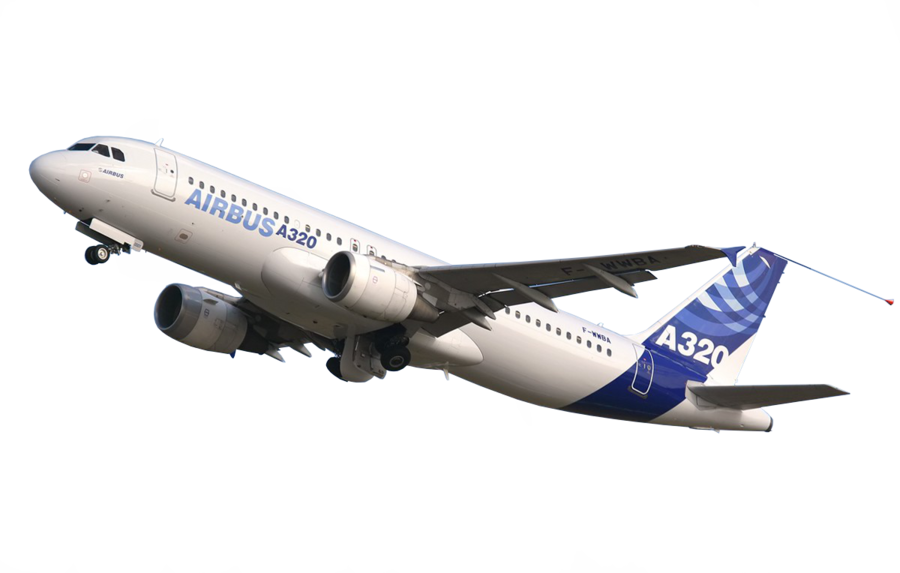
\includegraphics[width=1.1 cm,keepaspectratio]{aero/asd.png}}
%\usebackgroundtemplate{
\includegraphics[scale=0.45]{Selection_003}}

\lstdefinestyle{customc}{
  belowcaptionskip=1\baselineskip,
  breaklines=true,
  frame=L,
  xleftmargin=\parindent,
  language=C++,
  showstringspaces=false,
  basicstyle=\footnotesize\ttfamily,
commentstyle=\color{mygreen}, % comment color
    keywordstyle=\color{blue}, % keyword color
    stringstyle=\color{red} % string color
}





\lstset{escapechar=@,style=customc}

\newcommand{\includecode}[2][c]{\lstinputlisting{#2}<!---->}

\useinnertheme{rounded}
\begin{document}
\begin{frame}[plain]
\begin{picture}(0,0)(77.5,273)
\put(0,0){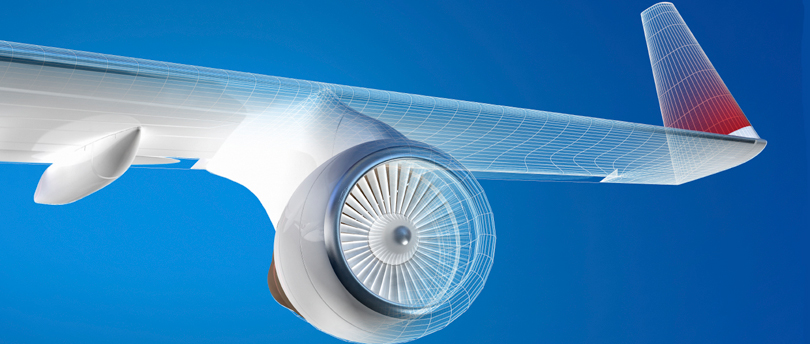
\includegraphics[height=3.4 cm,keepaspectratio,angle=90 ]{aero/mesh.jpg}}
\end{picture}
%\begin{picture}(0,0)(30.5,248)
   % \put(0,0){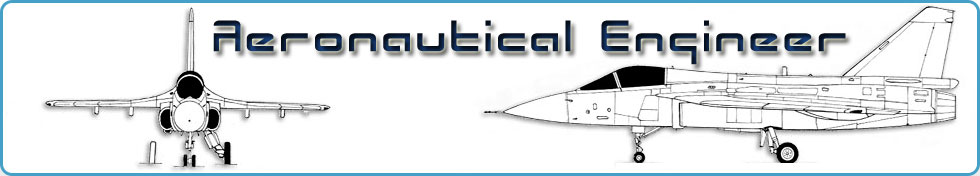
\includegraphics[height=1.5 cm,keepaspectratio]{aero/aero.jpg}}   
% \put(0,0){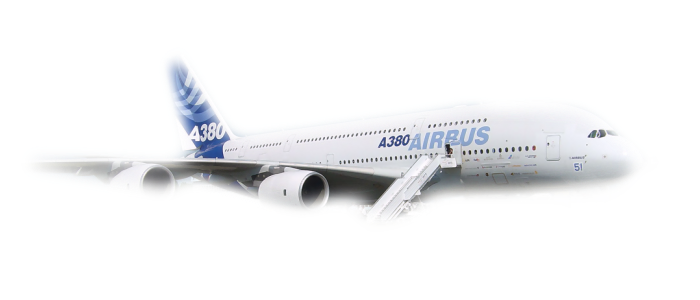
\includegraphics[height=4.3 cm,keepaspectratio ]{aero/airbus.png}}
%\end{picture}
         \titlepage
       \begin{figure}
    %\begin{center}
      
\includegraphics[scale=0.6]{figs/logo}
%\logo{
\includegraphics[scale=0.9]{logo.jpg}}
   % \end{center}
    \end{figure}
\end{frame}


\beamertemplatenavigationsymbolsempty
\setbeamertemplate{footline}[]

\newcommand\AtPagemyUpperLeft[1]{\AtPageLowerLeft{%
\put(\LenToUnit{0.8052\paperwidth},\LenToUnit{0.908\paperheight}){#1}}}
\AddToShipoutPictureFG{
  \AtPagemyUpperLeft{{
\includegraphics[width=2.5cm,keepaspectratio]{figs/logo.png}}}
}%



\begin{frame}[plain]
\begin{picture}(0,0)(79,228.5)
    \put(0,0){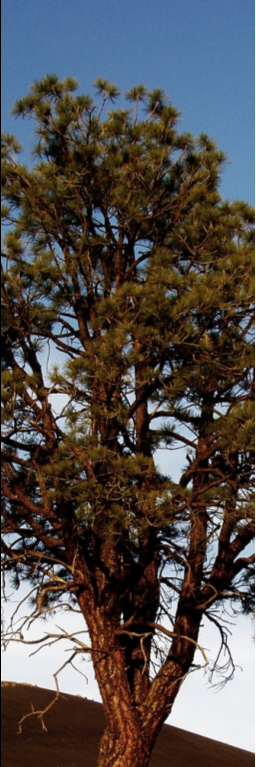
\includegraphics[width=2.3 cm,height=9.7 cm]{figs/Selection_008}}
\end{picture}
\frametitle{Outline}
\scriptsize{
\tableofcontents[currentsection,
    sectionstyle=show/show,
    subsectionstyle=show/show/hide]}
\end{frame}

\begin{frame}
\frametitle{Administration}
\framesubtitle{ Contact}
\begin{itemize}
  \item E-mail:  \href{mailto:qaziejazurrehman@gmail.com}{qaziejazurrehman@gmail.com} \footnote{ \href{mailto:qaziajazurrehman@gmail.com}{qaziajazurrehman@gmail.com}}
  \item Office hours: After 11:00 am
\end{itemize}
\end{frame}

\section{History}



\subsection{Introduction}
\begin{frame}
\frametitle{Introduction}
\framesubtitle{A Brief Introduction}
\begin{figure}[!tbp]
\centering
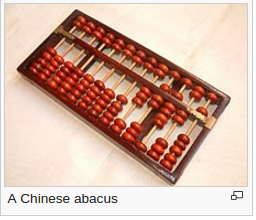
\includegraphics[scale = 0.55]{figs/Selection_002.png}
\end{figure}
\begin{itemize}
\item[\ding{45}] The only mechanical device that existed for numerical computation at the beginning of human history was the abacus, invented in Sumeria circa 2500 BC
\item[\ding{45}] And is still widely used by merchants, traders and clerks in Asia, Africa, and elsewhere
\end{itemize}
\end{frame}

\begin{frame}
\frametitle{Introduction}
\framesubtitle{Antikythera mechanism}
\begin{figure}[!tbp]
\centering
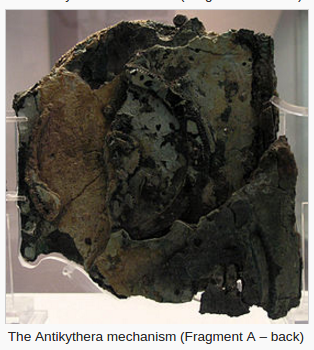
\includegraphics[scale = 0.35]{figs/bn.png}
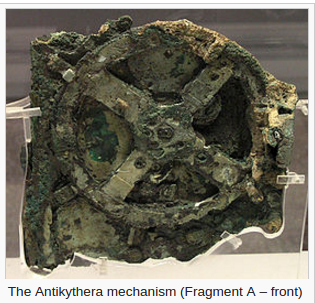
\includegraphics[scale = 0.4]{figs/bm.png}
\end{figure}
\small{
\begin{itemize}
\item[\ding{45}] The Antikythera mechanism, some time around 100 BC in ancient Greece, is the first known analog computer (mechanical calculator)
\item[\ding{45}] Designed to predict astronomical positions and eclipses for calendrical and astrological purposes as well as the Olympiads, the cycles of the ancient Olympic Games
\end{itemize}}
\end{frame}


\begin{frame}
\frametitle{Introduction}
\framesubtitle{$Badi'al-Zaman \ Ab\bar{u} \ al-'Izz \ Ism\bar{a}'\bar{i}l \newline ibn al-Raz\bar{a}z al-Jazar\bar{i}$}
\begin{itemize}
\item[\ding{45}] The Kurdish medieval scientist Al-Jazari built programmable automata\footnote{Same Idea as in Movie Automata (2014)} in 1206 AD.
\item Born: 1136 CE
\item Era: Islamic GOlden Age
\item Died: 1206 CE
\end{itemize}
\end{frame}

\begin{frame}
\frametitle{Introduction}
\framesubtitle{Johann Bernoulli \footnote{\url{http://en.wikipedia.org/wiki/Johann Bernoulli}}}
\begin{figure}[!tbp]
\centering
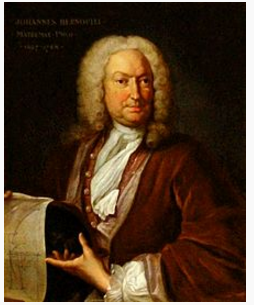
\includegraphics[scale = 0.35]{figs/Selection_0122.png}
\end{figure}
\begin{itemize}
\item 1667: Born in Switzerland, son of an apothecary
(in medical profession)
\item 1738: His son, Daniel Bernoulli published
\textit{Bernoulli's} principle
\item Students include his son Daniel, \em{\sc{Euler}}, L'Hopital
\item 1748: Death
\end{itemize}
\end{frame}

\begin{frame}
\frametitle{Introduction}
\framesubtitle{Leonhard Euler \tiny{\footnote{\url{ http://en.wikipedia.org/wiki/Leonhard Euler}}}}
\begin{figure}[!tbp]
\centering
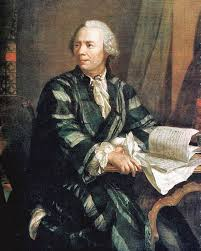
\includegraphics[scale = 0.35]{figs/download.jpg}
\end{figure}
\small{
\begin{itemize}
\item 1707: Born in Switzerland, son of a pastor
\item Among several other things, developed Euler's
identity, $e^{j\omega} = cos(\omega) + jsin(\omega)$
\item Also developed marvelous polyhedral fromula, nowadays written as "$v\ - \ e \ +\ f \ = \ 2$".
\item Friend of his doctoral advisor’s son, Daniel
Bernoulli, who developed Bernoulli’s principle
\item 1783: Death
\end{itemize}}
\end{frame}


\begin{frame}
\frametitle{Introduction}
\framesubtitle{Pierre-Simon Laplace \tiny{\footnote{http://en.wikipedia.org/wiki/Pierre-Simon Laplace}}}
\begin{figure}[!tbp]
\centering
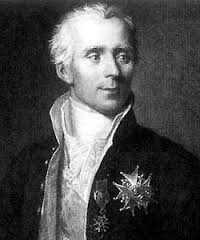
\includegraphics[scale = 0.35]{figs/zxc.jpg}
\end{figure}
\small{
\begin{itemize}
\item 1749: Born in France, son of a laborer
\item 1770-death: Worked on probability, celestial
mechanics, heat theory
\item 1785: Examiner, examined and passed Napoleon in
exam
\item 1790: Paris Academy of Sciences, worked with
Lavoisier, Coulomb
\item 1827: Died
\end{itemize}}
\end{frame}

\begin{frame}
\frametitle{Introduction}
\framesubtitle{Joseph Fourier \tiny{\footnote {\url{http://en.wikipedia.org/wiki/Joseph Fourier}}}}
\begin{figure}[!tbp]
\centering
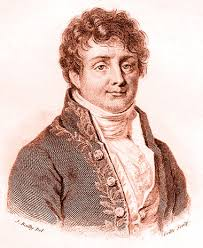
\includegraphics[scale = 0.35]{figs/cvb.jpg}
\end{figure}
\small{
\begin{itemize}
\item 1768: Born in France, son of a tailor
\item 1789-1799: Promoted the French Revolution
\item 1798: Went with Napoleon to Egypt and made
governor of Lower Egypt
\item 1822: Showed that representing a function by a
trigonometric series greatly simplifies the study of
heat propagation
\item1830: Fell from stairs and died shortly afterward
\end{itemize}}
\end{frame}



\begin{frame}
\frametitle{Introduction}
\framesubtitle{Charles Babbage}
\begin{figure}[!tbp]
\centering
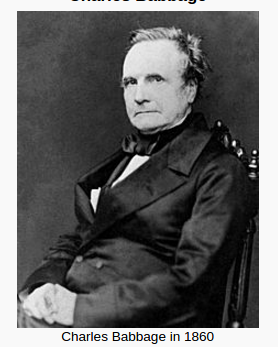
\includegraphics[scale = 0.35]{figs/Selection_006.png}
\end{figure}
\small{
\begin{itemize}
\item[\ding{45}]  Babbage is credited with inventing the first mechanical computer that eventually led to more complex designs.
\item Born: 26 December 1791 London, England   
\item Considered by some to be a "father of the computer"
\item Died: 18 October 1871 (aged 79) Marylebone, London, England
\end{itemize}}
\end{frame}

\begin{frame}
\frametitle{Introduction}
\framesubtitle{John Vincent Atanasoff (1903-1995)}
\begin{figure}[!tbp]
\centering
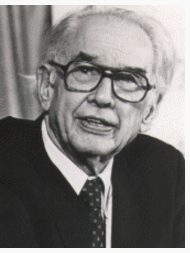
\includegraphics[scale = 0.5]{figs/Selection_01a2.png}
\caption[]{Atanasoff, in the 1990s.}
\end{figure}
Built first digital computer in the 1930s.
\end{frame}

\begin{frame}
\frametitle{Introduction}
\framesubtitle{Howard Hathaway Aiken (1901-1980)}
\begin{figure}[!tbp]
\centering
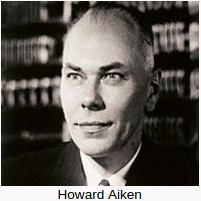
\includegraphics[scale = 0.5]{figs/Selection_01b2.png}
\end{figure}
\begin{itemize}
\item Built Mark I, during 1939-1944
\item Presented to public in 1944
\item Reaction was great
\begin{itemize}
\item Although Mark I meant a great deal for the development in
computer science, it's not recognised greatly today.
\item The reason for this is the fact that Mark I (and also Mark
II) was not electronic - it was electromagnetical
\end{itemize}
\end{itemize}
\end{frame}

\begin{frame}
\frametitle{Introduction}
\framesubtitle{J. Presper Eckert (1919-1995) and \\ Mauchly (1907-1980)}
\begin{figure}[!tbp]
\centering
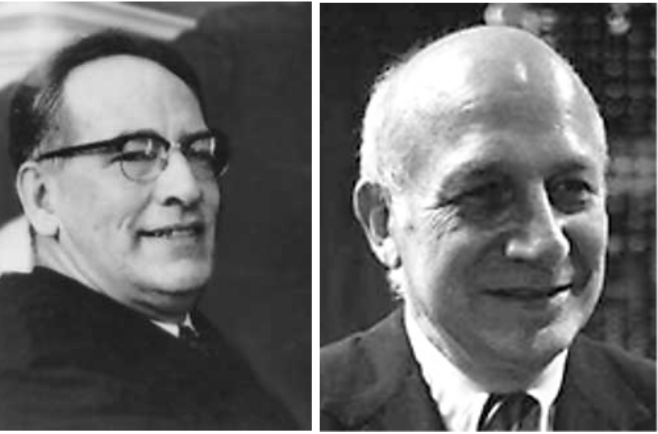
\includegraphics[scale = 0.31]{figs/Selection_01c2.png}
\end{figure}
Built ENIAC (Electronic Numerical Integrator and Computer), the first
electronic general-purpose computer during 1943-1945 at a cost of
\$468,000.
\end{frame}


\begin{frame}
\frametitle{Introduction}
\framesubtitle{Alan Mathison Turing\footnote{The Imitation Game: A 2014 Movie biographied on turing}}
\begin{figure}[!tbp]
\centering
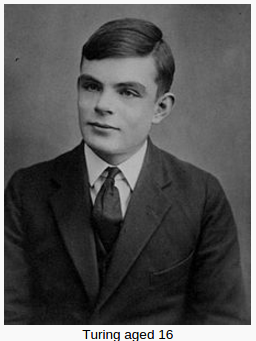
\includegraphics[scale = 0.35]{figs/alan.png}
\end{figure}
\begin{itemize}
\item {\bf Born}: 23 June 1912
\item Turing is widely considered to be the father of theoretical computer science and artificial intelligence
\item Famous for Breaking Enigma Machine Code
\item {\bf Died}: 7 June 1954 (aged 41)
\end{itemize}
\end{frame}

\begin{frame}
\frametitle{Turing Machine}
\begin{tikzpicture}
\tikzstyle{every path}=[very thick]

\edef\sizetape{0.7cm}
\tikzstyle{tmtape}=[draw,minimum size=\sizetape]
\tikzstyle{tmhead}=[arrow box,draw,minimum size=.5cm,arrow box
arrows={east:.25cm, west:0.25cm}]

%% Draw TM tape
\begin{scope}[start chain=1 going right,node distance=-0.15mm]
    \node [on chain=1,tmtape,draw=none] {$\ldots$};
    \node [on chain=1,tmtape] {};
    \node [on chain=1,tmtape] (input) {b};
    \node [on chain=1,tmtape] {b};
    \node [on chain=1,tmtape] {a};
    \node [on chain=1,tmtape] {a};
    \node [on chain=1,tmtape] {a};
    \node [on chain=1,tmtape] {a};
    \node [on chain=1,tmtape] {};
    \node [on chain=1,tmtape,draw=none] {$\ldots$};
    \node [on chain=1] {\textbf{\scriptsize{Input/Output Tape}}};
\end{scope}
%% Draw TM Finite Control
\begin{scope}
[shift={(3cm,-5cm)},start chain=circle placed {at=(-\tikzchaincount*60:1.5)}]
\foreach \i in {q_0,q_1,q_2,q_3,\ddots,q_n}
	\node [on chain] {$\i$};

% Arrow to current state
\node (center) {};
\draw[->] (center) -- (circle-2);

\node[rounded corners,draw=black,thick,fit=(circle-1) (circle-2) (circle-3) 
      (circle-4) (circle-5) (circle-6),
			label=below:\textbf{Finite Control}] (fsbox)
		{};
\end{scope}

%% Draw TM head below (input) tape cell
\node [tmhead,yshift=-.3cm] at (input.south) (head) {$q_1$};

%% Link Finite Control with Head
\path[->,draw] (fsbox.north) .. controls (4.5,-1) and (0,-2) .. node[right] 
			(headlinetext)
 			{} 
			(head.south);
\node[xshift=3cm] at (headlinetext)  
			{\begin{tabular}{c} 
				\textbf{Reading and Writing Head} \\  
				\textbf{(moves in both directions)} 
			 \end{tabular}};

\end{tikzpicture}
\end{frame}

\begin{frame}
\frametitle{History}
\framesubtitle{FORTRAN}
\begin{figure}[!tbp]
\centering
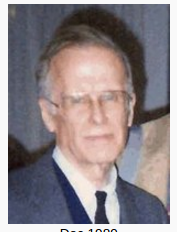
\includegraphics[scale = 0.35]{figs/Selection_007.png}
\end{figure}
\begin{itemize}
\item Inventor: John Backus
\item[\ding{45}]  FORTRAN, derived from Formula Translating System
\item It is a general-purpose, imperative programming language that is especially suited to numeric computation and scientific computing. Originally developed by IBM
\item First Appeared: 1957; 59 years ago
\end{itemize}
\end{frame}

\begin{frame}
\frametitle{History}
\framesubtitle{C++}
\begin{figure}[!tbp]
\centering
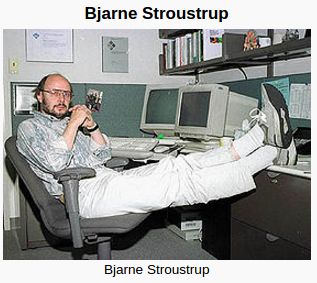
\includegraphics[scale = 0.35]{figs/cpr.png}
\end{figure}
\scriptsize{
\begin{itemize}
\item Inventor: Bjarne Stroustrup (at Bell Labs)
\item It is a general-purpose programming language. It has imperative, object-oriented and generic programming features, while also providing facilities for low-level memory manipulation
\item C++ is standardized by the International Organization for Standardization (ISO)
\item First Appeared: 1983; 33 years ago
\end{itemize}}
\end{frame}

\begin{frame}[shrink]%allowframebreaks]
\frametitle{Excellence of Human}
\framesubtitle{Equations: Changed The World}
\footnotesize{
 \resizebox{\linewidth}{!}{
%\begin{center}
\begin{tabular}{p{3.5cm} p{4.5cm} p{3cm}}
\\ \\ 
 \multicolumn{3}{c}{\textcolor{olive}{17 Equations That Changed The World}} \\ \\
 Pythagora.s Theorem&$a^2+b^2=c^2$&Pythagoras,530 BC\\
 Logarithms&$logxy=logx+logy$& John Napier, 1610\\
 Calculus &$\frac{df}{dt}=\lim_{h \to 0}\frac{f(t+h)-f(t)}{h}$& Newton, 1668\\
Law of Gravity   &$F=G\frac{m_1m_2}{r^2}$& Newton, 1687\\
Complex Identity&$i^2=-1$& Euler, 1750\\
Polyhedra Formula&$V-E+F=2$& Euler, 1751\\
Normal Distribution&$\phi(x)=\frac{1}{\sqrt{2\pi\rho}}e^\frac{(x-\mu)^2}{2\rho^2}$& C.F. Gauss, 1810\\
Wave Equation&$\frac{\partial^2u}{\partial t^2}=c^2\frac{\partial^2u}{\partial x^2}$& J. d'Almbert,1746\\
Fourier Transform&$f(\omega)=\int_{-\infty}^\infty f(x)e^{-2\pi ix\omega}dx$& J. Fourier, 1822\\
Navier-Stokes Equation&$\rho(\frac{\partial v}{\partial t}+v.\nabla v)=-\nabla p+\nabla .T+f$& C. Navier, G. Stokes, 1845\\
Maxwell's Equations& {\tiny{\begin{tabular}{c c}
$\nabla  E=\frac{\rho}{\epsilon 0}$ & $\nabla .H=0$ \\ 
$\nabla \times E=-\frac{1}{c}\frac{\partial H}{\partial t}$ & $\nabla \times H=\frac{1}{c}\frac{\partial E}{\partial t}$
\end{tabular}}}& J.C. Maxwell, 1865\\
Second Law of Thermosynamics &$dS\ge0$ & L. Boltzmann, 1874\\
Relativity & $E=mc^2$&Einstein, 1905\\
Schrodinger's Equation &$i\hslash\frac{\partial}{\partial t}\Psi=H\Psi$&E. Schrodinger, 1927\\
Information Theory &$H=-\sum p(x)logp(x)$&C. Shannon, 1949 \\
Chaos Theory &$x_{t+1}=kx_t(1-x_t)$& Robert May,1975\\
Black-Scholes\\ Equation&$\frac{1}{2}\sigma^2S^2\frac{\partial^2V}{\partial S^2}+rS\frac{\partial V}{\partial S}+\frac{\partial V}{\partial t}-rV=0$&F. Black, M. Scholes, 1990\\
\end{tabular}}}
%\end{center}}}
\end{frame}


\begin{frame}
\frametitle{Introduction}
\framesubtitle{Programming Accessories}
Whatever the approach to development may be, the final program must satisfy some fundamental properties. The following properties are among the most important
\begin{itemize}
\item[\ding{90}] Reliability
\item[\ding{90}] Robustness
\item[\ding{90}] Usability
\item[\ding{90}] Portability
\item[\ding{90}] Maintainability
\item[\ding{90}] Efficiency/performance
\end{itemize}
\end{frame}

%%%%%%%%%%%%%%%%%%%%%%%%%%%

\section{Labs}


%%%%%%%%%%%%%%%%%%%%%%%%%%%%%%%

\subsection{flowchart}

\begin{frame}[shrink]
\frametitle{Flow Chart}
\centering
\tikzstyle{startstop} = [rectangle, rounded corners, minimum width=1.8cm, minimum height=0.5cm,text centered, draw=black, fill=red!30]
\tikzstyle{io} = [trapezium, trapezium left angle=70, trapezium right angle=110, minimum width=1.8cm, minimum height=0.5cm, text centered, draw=black, fill=blue!30]
\tikzstyle{process} = [rectangle, minimum width=1.8cm, minimum height=0.6cm, text centered, draw=black, fill=orange!30]
\tikzstyle{decision} = [diamond, minimum width=1.2cm, minimum height=0.3cm, text centered, draw=black, fill=green!30]
\tikzstyle{arrow} = [thick,->,>=stealth]
\begin{center}
\tiny{
\begin{tikzpicture}[node distance=1.3cm]
\node (start) [startstop] {Start};
\node (in1) [io, below of=start] {Input};
\node (pro1) [process, below of=in1] {Process 1};
\node (dec1) [decision, below of=pro1] {Decision 1};
\node (pro2a) [process, below of=dec1, yshift=-0.15cm] {Process 2a};
\node (pro2b) [process, right of=dec1, xshift=2cm] {Process 2b};
\node (out1) [io, below of=pro2a] {Output};
\node (stop) [startstop, below of=out1] {Stop};
\draw [arrow] (start) -- (in1);
\draw [arrow] (in1) -- (pro1);
\draw [arrow] (pro1) -- (dec1);
\draw [arrow] (dec1) -- (pro2a);
\draw [arrow] (dec1) -- (pro2b);;
\draw [arrow] (dec1) -- node[anchor=east] {yes} (pro2a);
\draw [arrow] (dec1) -- node[anchor=south] {no} (pro2b);
\draw [arrow] (pro2a) -- (out1);
\draw [arrow] (out1) -- (stop);
\draw [arrow] (pro2b) |- (pro1);
\end{tikzpicture}}
\end{center}
\end{frame}

\begin{frame}[shrink]
\frametitle{Flow Chart}
\pagestyle{empty}

\centering
% Define block styles
\tikzstyle{decision} = [diamond, draw, fill=blue!20, 
    text width=4.5em, text badly centered, node distance=3cm, inner sep=0pt]
\tikzstyle{block} = [rectangle, draw, fill=blue!20, 
    text width=5em, text centered, rounded corners, minimum height=4em]
\tikzstyle{line} = [draw, -latex']
\tikzstyle{cloud} = [draw, ellipse,fill=red!20, node distance=3cm,
    minimum height=2em]
    
\begin{tikzpicture}[node distance = 2cm, auto]
    % Place nodes
    \node [block] (init) {initialize model};
    \node [cloud, left of=init] (expert) {expert};
    \node [cloud, right of=init] (system) {system};
    \node [block, below of=init] (identify) {identify candidate models};
    \node [block, below of=identify] (evaluate) {evaluate candidate models};
    \node [block, left of=evaluate, node distance=3cm] (update) {update model};
    \node [decision, below of=evaluate] (decide) {is best candidate better?};
    \node [block, below of=decide, node distance=3cm] (stop) {stop};
    % Draw edges
    \path [line] (init) -- (identify);
    \path [line] (identify) -- (evaluate);
    \path [line] (evaluate) -- (decide);
    \path [line] (decide) -| node [near start] {yes} (update);
    \path [line] (update) |- (identify);
    \path [line] (decide) -- node {no}(stop);
    \path [line,dashed] (expert) -- (init);
    \path [line,dashed] (system) -- (init);
    \path [line,dashed] (system) |- (evaluate);
\end{tikzpicture}

\end{frame}


\begin{frame}
\frametitle{\Large Computational Complexity Classes}
\tiny{
\begin{tikzpicture}
\pgftransformscale{.5}

%%% HELP LINES - uncomment to design/extend
% \draw[step=1cm,gray,very thin] (-10,0) grid (10,12);
% \node at (0,0) {\textbf{(0,0)}};

%% Horizontal bar
\draw[very thick] (10,0) -- (-10,0);

% LOG TIME
\draw (-1,0) parabola bend (0,2) (1,0) ;
\node at (0,1) {
	\begin{tabular}{c}
	LOG \\ Time
	\end{tabular}
};

% LOG SPACE
\draw (-2,0) parabola bend (0,3.5) (2,0);
\node at (0,2.5) {
	\begin{tabular}{c}
	LOG \\ Space
	\end{tabular}
};

% PTIME
\draw (-3,0) parabola bend (0,4.5) (3,0);
\node at (0,4) {PTIME};

% NP
\draw[dotted] (-4,0) parabola bend (2,6) (4.5,0);
\node[rotate=-45] at (3,3.5) {NPTIME};

% NP-complete
\node[circle,dotted,draw] at (2,5) {NPC};

% Co-NP
\draw[dashed] (4,0) parabola bend (-2,6) (-4.5,0);
\node[rotate=45] at (-2.5,4) {co-NPTIME};

% PSPACE
\draw (-6,0) parabola bend (0,7.2) (6,0);
\node at (0,6.5) {PSPACE};

% EXPTIME
\draw (-7,0) parabola bend (0,8.5) (7,0);
\node at (0,8) {EXPTIME};

% EXPTIME
\draw (-8,0) parabola bend (0,9.5) (8,0);
\node at (0,9) {EXPSPACE};

% ELEMENTARY
\draw (-9,0) parabola bend (0,11.5) (9,0);
\node at (0,10.5) {$\vdots$};
\node[anchor=north] at (0,11.4) {
	\begin{tabular}{c}
		ELEMENTARY \\
		$\vdots$ \\
		2EXPTIME
	\end{tabular}
};

% RECURSIVE
\draw[very thick] (-9.5,0) parabola bend (0,12.5) (9.5,0);
\node at (0,12) {MATLAB};
\end{tikzpicture}}
\end{frame}

\subsection{Lab Architecture}

\begin{frame}
\frametitle{Lab1}
\framesubtitle{Learn to Record and Share Your Results Electronically}
\begin{itemize}
\item Learn how to make a website and put your results on it
\begin{itemize}
\item Website files must not be path dependent, i.e, if I copy\
them to any location such as a USB, or different directory,
the website must still work
\item The main file of the website must be index.html
\end{itemize}
\item Many tools are available, but a good cross-platform open source
software is kompozer available from \url{http://www.kompozer.net/}
\end{itemize}
\end{frame}



\begin{frame}
\frametitle{Lab1}
\framesubtitle{Learn to Extend Existing Work in a Controls Topic}
Make groups, pick a research topic, create a website with following
headings:
\begin{enumerate}
\item Introduction
\item Technical Background
\item Expected Experiments
\item Expected Results
\item Expected Conclusions
\end{enumerate}
Present your website. Every group member will be quizzed randomly.
Your final work will count towards your lab exam.
\end{frame}



\section{Functions}


\begin{frame}
\frametitle{C++}
\framesubtitle{Functions}
\begin{itemize}
\item[\ding{36}] Functions allow to structure programs in segments of code to perform individual tasks.
\item[\ding{36}] A function is a group of statements that is given a name, and which can be called from some point of the program
\item[\ding{36}] {\small \textcolor{blue}{type} \textcolor{red}{name} (\textcolor{mygreen}{ parameter1, parameter2, ...}) \{ \textcolor{orange}{statements \}}}
\\ \vfill Where: \\
\begin{itemize}
\item[-] \textcolor{blue}{type} is the type of the value returned by the function.
\item[-] \textcolor{red}{name} is the identifier by which the function can be called.
\item[-] \textcolor{mygreen}{ parameters} each parameter consists of a type followed by an identifier, with each parameter being separated from the next by a comma.
\item[-]  \textcolor{orange}{statements} is the function's body. And specify what the function actually does.
\end{itemize}
\end{itemize}
\end{frame}

\begin{frame}
\frametitle{Functions}
\begin{tcolorbox}[title= ,width=11.5 cm]
\lstinputlisting[language=C++]{C++/9.cpp}
\end{tcolorbox}
\end{frame}


\begin{frame}
\frametitle{Functions}
\begin{tcolorbox}[title= ,width=9.85 cm]
\lstinputlisting[language=C++]{C++/7.cpp}
\end{tcolorbox}
\end{frame}




\begin{frame}
\frametitle{C++}
\framesubtitle{{\small Functions} \\ {\scriptsize Arguments passed by value and by reference }}
\begin{itemize}
\item[\ding{39}] In the functions seen earlier, arguments have always been passed by value.
\item[\ding{39}] This means what is passed to the function are the values of these arguments on the moment of the call
  \begin{itemize}
  \item[*] And are copied into the variables represented by the function parameters
  \end{itemize}
\item[\ding{39}] In certain cases, though, it may be useful to access an external variable from within a function. 
\begin{center}
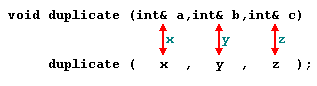
\includegraphics[width=8 cm,keepaspectratio]{figs/Selection_019.png}
\end{center}
\end{itemize}
\end{frame}

\begin{frame}
\frametitle{Functions}
\framesubtitle{Function with no type}
\begin{tcolorbox}[title= ,width=9.85 cm]
\lstinputlisting[language=C++]{C++/10.cpp}
\end{tcolorbox}
\end{frame}


\begin{frame}
\frametitle{C++}
\framesubtitle{{\small Functions} \\ {\scriptsize Efficiency considerations and const references}}
\begin{itemize}
\item Call by value
  \begin{itemize}
  \item[*] Values passed as aurgument are copied
    \begin{itemize}
     \item This is a relatively inexpensive operation for fundamental types such as $int$
     \item  An overhead occur if data is compound type \\
    \end{itemize}
  \end{itemize}
{\tiny \lstinputlisting[language=C++]{C++/n1.cpp}}
\end{itemize}

\end{frame}

\begin{frame}[shrink]
\frametitle{C++}
\framesubtitle{{\small Functions} \\ {\scriptsize Efficiency considerations and const references}}
    \begin{itemize} 
 \item Call by reference
    \begin{itemize}
\item[*] Overheading can be avoided
\begin{itemize}
\item  The function operates directly on the strings passed as arguments
\item  The functions with reference parameters are generally perceived as functions that modify the arguments passed \\

\end{itemize}
\end{itemize}
\pause
{\tiny \lstinputlisting[language=C++]{C++/n2.cpp}}
\end{itemize}
\pause
Defining arguments as constant can be used to prevent modifying the referenced arguments for function 
{\tiny \lstinputlisting[language=C++]{C++/n3.cpp}}
\noindent\makebox[\linewidth]{\rule{10 cm}{0.1pt}}
\textcolor{red}{Note: using \textcolor{blue}{const} will call this function by value in more efficient way }
\end{frame}




\subsubsection{Inline Function}
\begin{frame}
\frametitle{C++}
\framesubtitle{Inline Function}
\begin{itemize}
\item An optimized technique used by compiler to reduce the execution time \pause
  \item Compiler replaces the definition of inline functions at compile time instead of referring function definition at runtime \pause
  \item For big functions (in term of executable instruction), Compiler treat them as normal function
\end{itemize}
\end{frame}

\begin{frame}
\frametitle{C++}
\framesubtitle{Inline Function}
{\tiny \lstinputlisting[language=C++]{C++/12.cpp}}
\end{frame}

\begin{frame}
\frametitle{C++}
\framesubtitle{Inline Function}
{\tiny \lstinputlisting[language=C++]{C++/13.cpp}}
\end{frame}

\subsubsection{Overloads}
\begin{frame}
\frametitle{C++}
\framesubtitle{Overloaded Function}
\begin{itemize}[<+->]
\item In C++, two different functions can have the same name
\item But there arguments type should be different
\item Compiler determines by the type of argument being passed
\end{itemize}
\end{frame}

\begin{frame}[shrink]
\frametitle{C++}
\framesubtitle{Overloaded Function}
\begin{tcolorbox}[title= ,width=9.85 cm]
\tiny
\lstinputlisting[language=C++]{C++/17.cpp}
\end{tcolorbox}
\end{frame}


\begin{frame}[shrink]
\frametitle{C++}
\framesubtitle{Overloaded Function}
\begin{tcolorbox}[title= ,width=9.85 cm]
\tiny
\lstinputlisting[language=C++]{C++/18.cpp}
\end{tcolorbox}
\end{frame}

\subsubsection{Templates}
\begin{frame}
\frametitle{C++}
\framesubtitle{Templates}
\begin{itemize}[<+->]
\item The function could be overloaded for a lot of types (e.g previous slide)
\item And it could make sense for all of them to have the same body
\item C++ has the ability to define functions with generic types, known as function templates
\end{itemize}
\pause
\begin{tcolorbox}[title= ,width=9.85 cm]
\lstinputlisting[language=C++]{C++/19.cpp}
\end{tcolorbox}
\end{frame}


\begin{frame}[shrink]
\frametitle{C++}
\framesubtitle{Template Function}
\begin{tcolorbox}[title= ,width=11.85 cm]
\tiny
\lstinputlisting[language=C++]{C++/20.cpp}
\end{tcolorbox}
\end{frame}


\begin{frame}[shrink]
\frametitle{C++}
\framesubtitle{Template Function}
\begin{tcolorbox}[title= ,width=11.85 cm]
\tiny
\lstinputlisting[language=C++]{C++/21.cpp}
\end{tcolorbox}
\end{frame}

\begin{frame}[shrink]
\frametitle{C++}
\framesubtitle{Non-type template arguments}
\begin{tcolorbox}[title= ,width=11.85 cm]
\tiny
\lstinputlisting[language=C++]{C++/22.cpp}
\end{tcolorbox}
\end{frame}

\subsubsection{Name visibility}
\begin{frame}[shrink]
\frametitle{C++}
\framesubtitle{Scope (Local \& global) of variables}
\begin{itemize}[<+->]
\item The point in the program where variable declaration happens influences its visibility:
\item An entity declared outside any block has global scope
\item While an entity declared within a block (function or a selective statement), has block/local scope
\end{itemize}
\pause
\begin{tcolorbox}[title= ,width=9.85 cm]
\lstinputlisting[language=C++]{C++/23.cpp}
\end{tcolorbox}
\end{frame}

\subsubsection{Namespaces}
\begin{frame}[shrink]
\frametitle{C++}
\framesubtitle{Namespaces}
\begin{itemize}[<+->]
\item Non-local names bring more possibilities for name collision
\item Namespaces allow us to group named entities that otherwise would have global scope into narrower scopes,
\item This allows organizing the elements of programs into different logical scopes referred to by names
\end{itemize}
\pause
\begin{tcolorbox}[title= ,width=9.85 cm]
\lstinputlisting[language=C++]{C++/25.cpp}
\end{tcolorbox}
\end{frame}


\begin{frame}[shrink]
\frametitle{C++}
\framesubtitle{Namespaces}
\begin{tcolorbox}[title= ,width=11.85 cm]
\tiny
\lstinputlisting[language=C++]{C++/26.cpp}
\end{tcolorbox}
\end{frame}

\begin{frame}[shrink]
\frametitle{C++}
\framesubtitle{\textcolor{blue}{using} function}
The keyword \textcolor{blue}{using} introduces a name into the current declarative region (such as a block), thus avoiding the need to qualify the name. 
\pause
\begin{tcolorbox}[title= ,width=11.85 cm]
\tiny
\lstinputlisting[language=C++]{C++/27.cpp}
\end{tcolorbox}
\end{frame}

\begin{frame}[shrink]
\frametitle{C++}
\framesubtitle{\textcolor{blue}{using} \& \textcolor{blue}{namespace} function}
The keyword \textcolor{blue}{using}can also be used as a directive to introduce an entire \textcolor{blue}{namespace}:
\pause
\begin{tcolorbox}[title= ,width=11.85 cm]
\tiny
\lstinputlisting[language=C++]{C++/28.cpp}
\end{tcolorbox}
\end{frame}

\subsection{Array}
\begin{frame}
\frametitle{C++}
\framesubtitle{Array}
\begin{itemize}
\item An array is a series of elements of the same type placed in contiguous memory locations.
\item An array containing 5 integer values of type int called foo could be represented as:
\begin{figure}[!tbp]
\centering
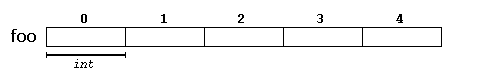
\includegraphics[scale = 0.5]{figs/Selection_020.png}
\end{figure}
\item An array must be declared before it is used. A typical declaration for an array in C++ is:
\pause
\begin{align*}
type \ &name[elements]; \pause \\
int \  foo[5] \quad &= \{16,\ 2,\ 77,\ 40,\ 12071 \};
\end{align*}

\begin{figure}[!tbp]
\centering
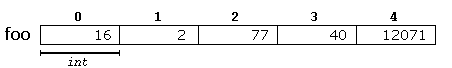
\includegraphics[scale = 0.5]{figs/Selection_021.png}
\end{figure}
\end{itemize}
\end{frame}

\begin{frame}
\frametitle{C++}
\framesubtitle{Array}
\begin{tcolorbox}[title= ,width=11.85 cm]
\lstinputlisting[language=C++]{C++/31.cpp}
\end{tcolorbox}
\end{frame}

\begin{frame}[shrink]
\frametitle{C++}
\framesubtitle{Multidimensional arrays}
\begin{itemize}[<+->]
\item Multidimensional arrays can be described as "arrays of arrays"
\item For example, a bidimensional array can be imagined as a two-dimensional table with elements of same uniform data type
\begin{figure}[!tbp]
\centering
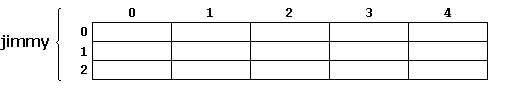
\includegraphics[scale = 0.5]{figs/Selection_022.png}
\end{figure}
\item The C++ syntax for this is: \\ \textcolor{orange}{int jimmy [3][5];}
\item Multidimensional arrays are not limited to two indices \\ \textcolor{orange}{char century [100][365][24][60][60];}
\item Multidimensional arrays are just an abstraction for programmers\\
\textcolor{orange}{int jimmy [3][5];}   // is equivalent to \\
\textcolor{orange}{int jimmy [15]; }    // (3 * 5 = 15)  
\end{itemize}
\end{frame}

\begin{frame}[fragile]
\frametitle{C++}
\framesubtitle{Multidimensional array}
{\tiny{
	\begin{columns}[t]
  		\begin{column}{5cm}
    			\begin{verbatim}
#define WIDTH 5
#define HEIGHT 3

int jimmy [HEIGHT][WIDTH];
int n,m;

int main ()
{
  for (n=0; n<HEIGHT; n++)
    for (m=0; m<WIDTH; m++)
    {
      jimmy[n][m]=(n+1)*(m+1);
    }
}
	\end{verbatim}
  		\end{column}
  		\begin{column}{5cm}
\begin{verbatim}
#define WIDTH 5
#define HEIGHT 3

int jimmy [HEIGHT * WIDTH];
int n,m;

int main ()
{
  for (n=0; n<HEIGHT; n++)
    for (m=0; m<WIDTH; m++)
    {
      jimmy[n*WIDTH+m]=(n+1)*(m+1);
    }
}
\end{verbatim}
  		\end{column}
	\end{columns}}}
\pause
\begin{itemize}[<+->]
\item Above (both) codes do not produce any output
\item But Assign values to the memory block called jimmy in the following way
\begin{figure}[!tbp]
\centering
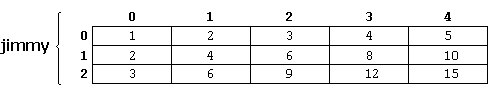
\includegraphics[scale = 0.5]{figs/Selection_023.png}
\end{figure}
\end{itemize}
\end{frame}



\begin{frame}[shrink]
\frametitle{C++}
\framesubtitle{Arrays as parameters}
\begin{itemize}[<+->]
\item To pass an array to a function as a parameter
\item In C++, it is not possible to pass the entire block of memory represented by an array to a function directly as an argument
\item But what can be passed instead is its address. As it is efficient way
\item To accept an array as parameter for a function 
\item The parameters can be declared as the array type, but with empty brackets, omitting the actual size of the array e.g. \\ \textcolor{orange}{void procedure (int arg[])
\\ int myarray [40]; \\procedure (myarray);}

\end{itemize}
\end{frame}


\begin{frame}
\frametitle{C++}
\framesubtitle{Arrays as parameters}
\begin{tcolorbox}[title= ,width=11.85 cm]
\lstinputlisting[language=C++]{C++/32.cpp}
\end{tcolorbox}
\end{frame}


\begin{frame}
\frametitle{C++}
\framesubtitle{Library arrays}
\begin{itemize}[<+->]
\item The arrays explained above are directly implemented as a language feature
\item Restricting its copy and easily decay into pointers, they probably suffer from an excess of optimization
\item C++ provides an alternative array type as a standard container (a type template (a class template, in fact))
\item To accept an array as parameter for a function 
\item The parameters can be declared as the array type, but with empty brackets, omitting the actual size of the array e.g. \\ \textcolor{orange}{void procedure (int arg[])
\\ int myarray [40]; \\procedure (myarray);}
\end{itemize}
\end{frame}

\begin{frame}[fragile]
\frametitle{C++}
\framesubtitle{language built-in array Vs container library array}
\tiny
	\begin{columns}[t]
  		\begin{column}{5cm}
    			\begin{verbatim}
#include <iostream>

using namespace std;

int main()
{
  int myarray[3] = {10,20,30};

  for (int i=0; i<3; ++i)
    ++myarray[i];

  for (int elem : myarray)
    cout << elem << '\n';
}
	\end{verbatim}
  		\end{column}
  		\begin{column}{5cm}
\begin{verbatim}
#include <iostream>
#include <array>
using namespace std;

int main()
{
  array<int,3> myarray {10,20,30};

  for (int i=0; i<myarray.size(); ++i)
    ++myarray[i];

  for (int elem : myarray)
    cout << elem << '\n';
}
\end{verbatim}
  		\end{column}
	\end{columns}
\end{frame}


\section{Dynamic Memory}
\begin{frame}
\frametitle{C++}
\framesubtitle{Dynamic Memory}
\begin{itemize}[<+->]
\item In previous programs all memory needs were determined before program execution by defining the variables 
\item But when the memory needed depends on user input.
\item On these cases, programs need to dynamically allocate memory
\begin{itemize}
\item Dynamic memory is allocated using operator \textcolor{blue}{new}
\item  \textcolor{blue}{new} is followed by a data type specifier 
\end{itemize}
\item If a sequence of more than one element is required, the number of these within brackets []. 
\item It returns a pointer to the beginning of the new block of memory allocated.\\
\textcolor{orange}{pointer = new type \\
pointer = new type [number\_of\_elements]}
\end{itemize}
\textcolor{mygreen}{
int * foo;\\
foo = new int [5];}
\end{frame}

\subsection{Dynamic Memory}
\begin{frame}
\frametitle{C++}
\framesubtitle{Dynamic Memory}
\begin{itemize}[<+->]
\item C++ provides two standard mechanisms to check if the allocation was successful:
\begin{itemize}
\item[*] One is by handling exceptions i.e.(exception of type bad\_alloc is thrown when the allocation fails.)
\begin{itemize}
\item This exception method is the method used by default by \textcolor{blue}{new}
\begin{center}foo = \textcolor{blue}{new int} [5]; \end{center}
\end{itemize}

\item[*]  The other method is known as nothrow (the pointer returned by new is a null pointer) 
\begin{itemize}
\item On failure, memory is not thrown over bad\_alloc
\begin{center}foo = \textcolor{blue}{new} (nothrow) \textcolor{blue}{int} [5]; \end{center}
\end{itemize}
\end{itemize}
\item Failure is detected by null pointer
\lstinputlisting[language=C++]{C++/35.cpp}
\end{itemize}
\end{frame}

\begin{frame}
\frametitle{C++}
\framesubtitle{Erasing Pointers}
\begin{itemize}[<+->]
\item Memory allocated dynamically is only needed during specific periods of time within a program
\item  To free memory allocated dynamically $operator$ delete is used
\begin{center}
\textcolor{blue}{
delete} pointer; \\
\textcolor{blue}{delete}[] pointer;
\end{center}
\end{itemize}

Note :
\only<3>{\textcolor{red}{ The first statement releases the memory of a single element allocated using new}}
\only<4>{\textcolor{mygreen}{ The second one releases the memory allocated for arrays of elements using new and a size in brackets ([]).}}
\end{frame}

\begin{frame}[shrink]
\frametitle{C++}
\framesubtitle{Dynamic Memory}
\lstinputlisting[language=C++]{C++/36.cpp}

\end{frame}

\section{Structure}

\begin{frame}
\frametitle{C++}
\framesubtitle{Structure}
\begin{itemize}[<+->]
\item A data structure is a group of data elements grouped together under one name
\item These data elements, known as members, can have different types and different lengths
\item syntax is
\item[]  struct type\_name { \\
member\_type1 member\_name1;\\
member\_type2 member\_name2;\\
member\_type3 member\_name3;\\
.\\
.\\
} object\_names;
\end{itemize}
\end{frame}

\begin{frame}[fragile]
\frametitle{C++}
\framesubtitle{Structure}
{{
	\begin{columns}[t]
  		\begin{column}{5cm}
    			\begin{verbatim}
struct product {
  int weight;
  double price;
} ;

product apple;
product banana, melon;
	\end{verbatim}
  		\end{column}
  		\begin{column}{5cm}
\begin{verbatim}
struct product {
  int weight;
  double price;
} apple, banana, melon;
\end{verbatim}
  		\end{column}
	\end{columns}}}
\vfil
\bigskip
\underline{Note: } \\
It is important to clearly differentiate between \\
\only<1> {what is the \alert{structure type} name (product),}
\only<2> {what is an object of this \alert{type (apple, banana, and melon)}}
\end{frame}

\begin{frame}
\frametitle{C++}
\framesubtitle{Important Characters}
\footnotesize
\begin{tabular}{|c|c|c|}
\hline 
Expression &What is evaluated &Equivalent \\
\hline
a.b &Member b of object a &\\ \hline 
a->b&Member b of object pointed to by a&(*a).b \\ \hline
*a.b&Value pointed to by member b of object a&*(a.b)  \\ \hline
\end{tabular}
\end{frame}



\begin{frame}
\frametitle{C++}
\framesubtitle{Nested Structure}

\lstinputlisting[language=C++]{C++/40.cpp}


\lstinputlisting[language=C++]{C++/41.cpp}

\end{frame}

\section{Classes}
\subsection{Introduction}

\begin{frame}
\frametitle{C++}
\framesubtitle{Classes}
\small
\begin{itemize}[<+->]
\item Classes are an expanded concept of data structures:
\item They can contain data members, but they can also contain functions as members.
\item Classes are defined using either keyword class or keyword struct, syntax is:
\item[]  \textcolor{blue}{class class\_name { \\
  access\_specifier\_1:\\
    member1;\\
  access\_specifier\_2:\\
    member2;\\
  ...\\
} object\_names;}
\item Classes have new things called access specifiers. And is one of the following three keywords:\textcolor{blue}{ private, public or protected}
\item Classes can be defined not only with keyword class, but also with keywords \textcolor{red}{struct} and \textcolor{red}{union}.
\end{itemize}
\end{frame}


\begin{frame}
\frametitle{C++}
\framesubtitle{Access Specifiers}
\begin{itemize}[<+->]
\item \textcolor{blue}{private members} of a class are accessible only from within other members of the same class (or from their "friends").
\item  \textcolor{blue}{protected members} are accessible from other members of the same class (or from their "friends"), but also from members of their derived classes.
\item Finally,  \textcolor{blue}{public members} are accessible from anywhere where the object is visible.
\item By default, all members of a class declared with the class keyword have  \textcolor{blue}{private} access for all its members
\end{itemize}
\lstinputlisting[language=C++]{C++/new.cpp}
\end{frame}


\begin{frame}[shrink]
\frametitle{Classes}
\begin{tcolorbox}[title= ,width=9.85 cm]
\scriptsize
\lstinputlisting[language=C++]{C++/42.cpp}
\end{tcolorbox}
\end{frame}


\begin{frame}[shrink]
\frametitle{Classes}
\framesubtitle{Multiple Type}
\only<1>{
\begin{itemize}
\item The most important property of a class is that it is a type
\item we can declare multiple objects of it.
\item For example, following with the previous example of class Rectangle, we could have declared the object rectb in addition to object rect:
\end{itemize}}
\only<2>{
\begin{tcolorbox}[title= ,width=14.85 cm]
\small
\lstinputlisting[language=C++]{C++/43.cpp}
\end{tcolorbox}}
\end{frame}

\subsection{Constructors}

\begin{frame}
\frametitle{Classes}
\framesubtitle{Constructors}
\begin{itemize}[<+->]
\item \textcolor{red}{What would happen in the previous example if we called the member function area before having called \textcolor{mygreen}{set\_values?} }
\item An undetermined result, since the members \textcolor{blue}{width} and \textcolor{blue}{height} had never been assigned a value.
\item In order to avoid that, a class can include a special function called its  \textcolor{blue}{constructors}
\item The Rectangle class above can easily be improved by implementing a constructor
\end{itemize}
\end{frame}


\begin{frame}[shrink]
\frametitle{Classes}
\framesubtitle{Constructors}
\begin{tcolorbox}[title= ,width=14.85 cm]
\scriptsize
\lstinputlisting[language=C++]{C++/44.cpp}
\end{tcolorbox}
\end{frame}


\begin{frame}
\frametitle{Classes}
\framesubtitle{Overloading Constructors}
\begin{itemize}[<+->]
\item A constructor can also be overloaded with \only<1>{\textcolor{orange}{different versions taking different parameters}}
\only<2> {\textcolor{cyan}{a different number of parameters and/or parameters of different types}}
\item The compiler will automatically call the one whose parameters match the arguments
\end{itemize}
\end{frame}


\begin{frame}[shrink]
\frametitle{Classes}
\framesubtitle{Overloading Constructors}
\begin{tcolorbox}[title= ,width=14.85 cm]
\scriptsize
\lstinputlisting[language=C++]{C++/45.cpp}
\end{tcolorbox}
\end{frame}


\begin{frame}[shrink]
\frametitle{Classes}
\framesubtitle{Uniform Initialization}
\begin{itemize}[<+->]
\item The way of calling constructors by enclosing their arguments in parentheses, as shown above, is known as $functional \ form$
\item \textcolor{blue}{class\_name object\_name = initialization\_value;}\\ 
\item \textcolor{blue}{class\_name object\_name \{ value, value, value, ... \}}
\end{itemize}
\pause
\scriptsize
\lstinputlisting[language=C++]{C++/46.cpp}
\end{frame}


\begin{frame}[shrink]
\frametitle{Classes}
\framesubtitle{Member initialization in constructors}
\begin{tcolorbox}[title= ,width=14.85 cm]
\scriptsize
\lstinputlisting[language=C++]{C++/47.cpp}
\end{tcolorbox}
\end{frame}


\section{File I/O}

\subsection{File I/O}

\begin{frame}[fragile]
\frametitle{File Input/Output}
\begin{itemize}[<+->]
\item C++ provides the following classes to perform output and input of characters to/from files
\begin{itemize}[<+->]
\item \alert{\textcolor{red}{ofstream}}: Stream class to write on files
\item  \alert{\textcolor{red}{ifstream}}: Stream class to read from files
\item  \alert{\textcolor{red}{fstream}}: Stream class to both read and write from/to files.
\end{itemize}
\item These classes are derived directly or indirectly from the classes \textcolor{blue}{istream} and \textcolor{blue}{ostream}
\end{itemize}
\lstinputlisting[language=C++]{C++/48.cpp}
\end{frame}


\begin{frame}
\frametitle{File Input/Output}
\framesubtitle{Open a file}
\begin{itemize}[<+->]
\item In order to open a file with a stream object we use its member function open:
\begin{itemize}[<+->]
\item \alert{\textcolor{red}{open (filename, mode);}}
\end{itemize}
\item Filename is a string representing the name of the file to be opened
\item Mode is an optional parameter with a combination of the following flag
\end{itemize}
\scriptsize{
\begin{tabular}{| l | l |}
\hline 
ios::in	&Open for input operations. \\ \hline
ios::out	&Open for output operations.\\ \hline
ios::binary &Open in binary mode.\\ \hline
ios::ate	&Set the initial position at the end of the file.\\
                &If this flag is not set, the initial position is the beginning of the file.\\ \hline
ios::app	&All output operations are performed at the end of the file, \\
               &appending the content to the current content of the file.\\ \hline
ios::trunc	&If the file is opened for output operations and it already existed,\\
                  &its previous content is deleted and replaced by the new one. \\ \hline
\end{tabular}}
\lstinputlisting[language=C++]{C++/np5.cpp}
\end{frame}

\begin{frame}
\frametitle{File Input/Output}
\framesubtitle{Open a file}
\scriptsize
\begin{itemize}[<+->]
\item classes ofstream, ifstream and fstream has a default mode that is used if the file is opened without a second argument: \\
\scriptsize{
\begin{tabular}{| l | l |}
\hline 
{\bf class}	 &{\bf default mode parameter} \\ \hline
ofstream	&ios::out \\ \hline
ifstream	&ios::in \\ \hline
fstream	&ios::in | ios::out \\ \hline
\end{tabular}}
\item File streams opened in binary mode perform input and output operations independently of any format considerations
\item Non-binary files are known as text files \\
\lstinputlisting[language=C++]{C++/np6.cpp} 
\item To check if a file stream was successful opening a file,use $is\_open$ \\
\lstinputlisting[language=C++]{C++/np7.cpp}
\item Closing a file \\ 	 myfile.close();
\end{itemize}
\end{frame}

\subsection{fileopen}

\begin{frame}
\frametitle{Text files}
\framesubtitle{Writing}
Writing operations on text files are performed in the same way we operated with cout:
\begin{tcolorbox}[title= ,width=14.85 cm]
\scriptsize
\lstinputlisting[language=C++]{C++/49.cpp}
\end{tcolorbox}
\end{frame}

\begin{frame}[shrink]
\frametitle{Text files}
\framesubtitle{Reading}
Reading from a file can also be performed in the same way that we did with cin:
\begin{tcolorbox}[title= ,width=14.85 cm]
\scriptsize
\lstinputlisting[language=C++]{C++/50.cpp}
\end{tcolorbox}
\end{frame}


\subsection{State flags}

\begin{frame}
\frametitle{File Input/Output}
\framesubtitle{Checking state flags}
\scriptsize
The following member functions exist to check for specific states of a stream (all of them return a bool value): 
\begin{itemize}[<+->]
\item \alert{bad()}\\
Returns true if a reading or writing operation fails. For example, in the case that we try to write to a file that is not open for writing or if the device where we try to write has no space left.
 \item \alert{fail()}\\
Returns true in the same cases as bad(), but also in the case that a format error happens, like when an alphabetical character is extracted when we are trying to read an integer number.
\item \alert{eof()}\\
Returns true if a file open for reading has reached the end.
\item \alert{good()}\\
It is the most generic state flag: it returns false in the same cases in which calling any of the previous functions would return true. Note that good and bad are not exact opposites (good checks more state flags at once).
\end{itemize}
The member function \alert{clear()} can be used to reset the state flags.
\end{frame}



\begin{frame}
\frametitle{File Input/Output}
\framesubtitle{get and put stream positioning}
\scriptsize
The following member functions exist to check for specific states of a stream (all of them return a bool value): 
\begin{itemize}[<+->]
\item All i/o streams objects keep internally -at least- one internal position:
\item ifstream, like istream, keeps an internal get position with the location of the element to be read in the next input operation.
\item ofstream, like ostream, keeps an internal put position with the location where the next element has to be written.
\item Finally, fstream, keeps both, the get and the put position, like iostream.
\end{itemize}

\alert{tellg()} and \alert{tellp()}\\
These two member functions with no parameters return a value of the member type streampos, which is a type representing the current get position (in the case of tellg) or the put position (in the case of tellp).\\

\alert{seekg()} and \alert{seekp()}\\
These functions allow to change the location of the get and put positions. Both functions are overloaded with two different prototypes. The first form is:\\
\alert{seekg ( position );}\\
\alert{seekp ( position );}
\end{frame}



\begin{frame}[shrink]
\frametitle{Text files}
\begin{tcolorbox}[title= ,width=14.85 cm]
\scriptsize
\lstinputlisting[language=C++]{C++/51.cpp}
\end{tcolorbox}
Notice the type we have used for variables begin and end:\\ 
streampos size;
\end{frame}

\subsection{Binary}


\begin{frame}
\frametitle{File Input/Output}
\framesubtitle{Binary}
\scriptsize
The following member functions exist to check for specific states of a stream (all of them return a bool value): 
\begin{itemize}[<+->]
\item File streams include two member functions specifically designed to read and write binary data sequentially: \alert{write} and  \alert{read}
\item \alert{write} is a member function of ostream (inherited by ofstream). 
\item \alert{read} is a member function of istream (inherited by ifstream)
\end{itemize}
\lstinputlisting[language=C++]{C++/np9.cpp}
\end{frame}



\begin{frame}[shrink]
\frametitle{Text files}
\lstinputlisting[language=C++]{C++/52.cpp}
\end{frame}


%%%%%%%%%%%%%%%%%%%%%%%%%%%%%%%%%%%%%%%%%


\section{Codes}
\subsection{For loop}

\begin{frame}
\frametitle{for loop}
\begin{tcolorbox}[title= ,width=9.85 cm]
\lstinputlisting[language=C++]{C++/0b.cpp}
\end{tcolorbox}
\end{frame}

\begin{frame}
\frametitle{for loop}
\begin{tcolorbox}[title= ,width=9.85 cm]
\lstinputlisting[language=C++]{C++/0a.cpp}
\end{tcolorbox}
\end{frame}

\begin{frame}
\frametitle{for loop}
\begin{tcolorbox}[title=Custom Count Down,width=9.85 cm]
\lstinputlisting[language=C++]{C++/0.cpp}
\end{tcolorbox}
\end{frame}

\subsection{while loop}
\begin{frame}
\frametitle{While Loop}
\begin{tcolorbox}[title=Custom Count Down,width=9.85 cm]
\lstinputlisting[language=C++]{C++/1.cpp}
\end{tcolorbox}
\end{frame}

\begin{frame}
\frametitle{do-while loop}
\begin{tcolorbox}[title=   ,width=9.85 cm]
\lstinputlisting{C++/2.cpp}
\end{tcolorbox}
\end{frame}

\subsection{break statement}

\begin{frame}
\frametitle{break statement}
\begin{tcolorbox}[title=,width=9.85 cm]
\lstinputlisting{C++/3.cpp}
\end{tcolorbox}
\end{frame}

\subsection{continue statement}

\begin{frame}
\frametitle{continue statement}
\begin{tcolorbox}[title= ,width=9.85 cm]
\lstinputlisting{C++/4.cpp}
\end{tcolorbox}
\end{frame}

\subsection{go-to statement}

\begin{frame}
\frametitle{go-to statement}
\scriptsize{
\begin{tcolorbox}[title=  ,width=9.85 cm]
\lstinputlisting{C++/5.cpp}
\end{tcolorbox}}
\end{frame}

\subsection{Switch statement}

\begin{frame}
\frametitle{Switch statement}
\scriptsize{
\begin{tcolorbox}[title=  ,width=9.85 cm]
\lstinputlisting{C++/6.cpp}
\end{tcolorbox}}
\end{frame}

\subsection{function}

\begin{frame}[shrink]
\frametitle{functions}
\begin{tcolorbox}[title= ,width=11.5 cm]
\lstinputlisting[language=C++]{C++/8.cpp}
\end{tcolorbox}
\end{frame}

\begin{frame}[shrink]
\frametitle{functions}
\framesubtitle{Default Values}
\begin{tcolorbox}[title= ,width=11.5 cm]
\lstinputlisting[language=C++]{C++/14.cpp}
\end{tcolorbox}
\end{frame}

\begin{frame}[shrink]
\frametitle{functions}
\begin{tcolorbox}[title= ,width=15.5 cm]
\lstinputlisting[language=C++]{C++/15.cpp}
\end{tcolorbox}
\end{frame}

\begin{frame}[shrink]
\frametitle{functions}
\framesubtitle{Recursivity}
\begin{tcolorbox}[title= ,width=15.5 cm]
\lstinputlisting[language=C++]{C++/16.cpp}
\end{tcolorbox}
\end{frame}

\begin{frame}[shrink]
\frametitle{Scope}
\framesubtitle{global \& local variable}
\begin{tcolorbox}[title= ,width=15.5 cm]
\lstinputlisting[language=C++]{C++/24.cpp}
\end{tcolorbox}
\end{frame}


\subsection{namespace}
\begin{frame}[shrink]
\frametitle{Scope}
\framesubtitle{namespace}
\begin{tcolorbox}[title= ,width=15.5 cm]
\lstinputlisting[language=C++]{C++/29.cpp}
\end{tcolorbox}
\end{frame}

\begin{frame}
\frametitle{Scope}
\framesubtitle{namespace}
\begin{tcolorbox}[title= ,width=15.5 cm]
\lstinputlisting[language=C++]{C++/30.cpp}
\end{tcolorbox}
\end{frame}

\subsection{Array}


\begin{frame}[shrink]
\frametitle{Array}
\framesubtitle{string, dimensional}
\begin{tcolorbox}[title= ,width=15.5 cm]
\lstinputlisting[language=C++]{C++/33.cpp}
\end{tcolorbox}
\end{frame}

\begin{frame}
\frametitle{Array}
\framesubtitle{string, dimensional}
\begin{tcolorbox}[title= ,width=15.5 cm]
\lstinputlisting[language=C++]{C++/34.cpp}
\end{tcolorbox}
\end{frame}

\subsection{Structure}

\begin{frame}[shrink]
\frametitle{Structure\attachfile{C++/37.cpp}}
\framesubtitle{Basic}
\begin{tcolorbox}[title= ,width=15.5 cm]
\lstinputlisting[language=C++]{C++/37.cpp}
\end{tcolorbox}
\end{frame}

\begin{frame}[shrink]
\frametitle{Structure\attachfile{C++/38.cpp}}
\framesubtitle{Pointers}
\begin{tcolorbox}[title= ,width=15.5 cm]
\lstinputlisting[language=C++]{C++/38.cpp}
\end{tcolorbox}
\end{frame}

\begin{frame}[shrink]
\frametitle{Structure\attachfile{C++/39.cpp}}
\framesubtitle{Pointers}
\begin{tcolorbox}[title= ,width=15.5 cm]
\lstinputlisting[language=C++]{C++/39.cpp}
\end{tcolorbox}
\end{frame}


%%%%%%%%%%%%%%%%

\centering
     \begin{frame}[plain]
           \vspace{2cm}
          \begin{picture}(0,0)(170,170)
          \put(0,0){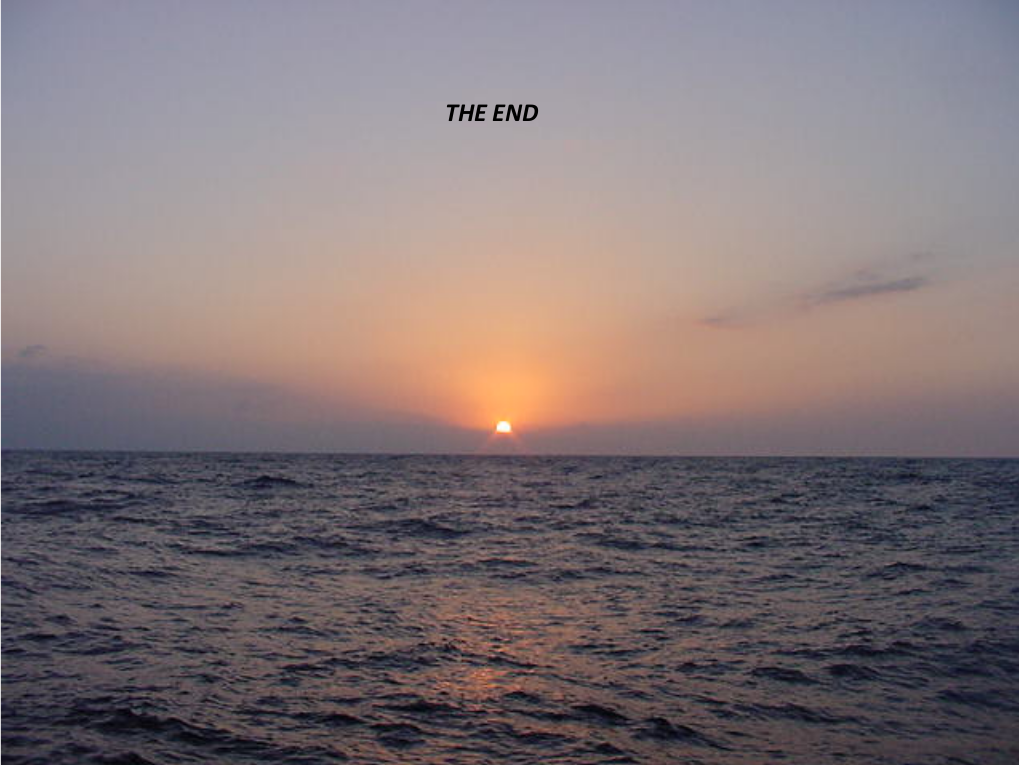
\includegraphics[width=13 cm,height=9.7 cm]{figs/thank.png}}
         \end{picture}
                  {\huge {Thank you}} % Huge makes the text size, well, Huge
           \vspace{3cm}
           \begin{flushright}
                 \href{mailto:qaziajazurrehman@gmail.com}{\textcolor{white}{Email}}
           \end{flushright}
       \end{frame}
\end{document}
